\documentclass[a4paper,12pt]{report}

\usepackage[]{fullpage}
\usepackage{graphics}
\usepackage[hidelinks]{hyperref}
\usepackage{etaremune}
\usepackage{graphicx}
\usepackage{rotating}
\usepackage{color}
\usepackage{xcolor}
\usepackage{standalone}
\usepackage{adjustbox}
%\usepackage{palatino} %Font package

\setlength{\parindent}{0em}
\setlength{\parskip}{1em}

% Title Page
\title{
\begin{center}
\begin{normalsize}
 
\includegraphics[width=0.5\textwidth]{USIU.png}\\
\textbf{}\end{normalsize}\\
\vspace{1in}
\textbf{MIS 6040 - NETWORKING AND WIRELESS COMMUNICATIONS} \\
\vspace*{\fill}
\author{Arthur Buliva\\645381\\\begin{small}abuliva@usiu.ac.ke\end{small}}
	\begin{footnotesize}
		\textbf{ASSIGNMENT I}
		\vspace{1in}
	\end{footnotesize}
\end{center}
}

\begin{document}
\maketitle

\section*{Explain criteria of measuring effectiveness of a data communication system in detail.}
The effectiveness of any data communications system depends
upon the following four fundamental characteristics:
\begin{enumerate}
\item Delivery: The data should be delivered to the correct
destination and correct user.
\item Accuracy: The communication system should deliver the data
accurately, without introducing any errors. The data may get
corrupted during transmission affecting the accuracy of the
delivered data.
\item Timeliness: Audio and Video data has to be delivered in a
timely manner without any delay; such a data delivery is called
real time transmission of data.
\item Jitter: It is the variation in the packet arrival time. Uneven Jitter
may affect the timeliness of data being transmitted.
\end{enumerate}

\section*{Explain 5 components of a data communication system in detail.}
\begin{enumerate}
\item Message
Message is the information to be communicated by the sender to the receiver.
\item Sender
The sender is any device that is capable of sending the data (message).
\item Receiver
The receiver is a device that the sender wants to communicate the data (message).
\item Transmission Medium
It is the path by which the message travels from sender to receiver. It can be wired or wireless and many subtypes in both.
\item Protocol
It is an agreed upon set or rules used by the sender and receiver to communicate data.
A protocol is a set of rules that governs data communication. A Protocol is a necessity in data communications without which the communicating entities are like two persons trying to talk to each other in a different language without know the other language.
\end{enumerate}

\section*{Explain data representation in detail.}
Data is collection of raw facts which is processed to deduce information.
There may be different forms in which data may be represented.
Some of the forms of data used in communications are as follows:
\begin{enumerate}
\item Text
Text includes combination of alphabets in small case as well as upper case.
It is stored as a pattern of bits. Prevalent encoding system : ASCII, Unicode
\item Numbers
Numbers include combination of digits from 0 to 9.
It is stored as a pattern of bits. Prevalent encoding system : ASCII, Unicode
\item Images
Commonly used Image formats : jpg, png, bmp, etc
\item Audio
Data can also be in the form of sound which can be recorded and broadcasted. Example: What we hear on the radio is a source of data or information. Audio data is continuous, not discrete.
\item Video
Video refers to broadcasting of data in form of picture or movie
\end{enumerate}

\section*{Explain types of data flow in detail.}
Any two devices will communicate with each other by sending and receiving data. The data can move in between the two devices in the following ways.

\begin{enumerate}
\item  Simplex. Communication is unidirectional. Only one of the devices sends the data and the other one only receives the data at any given time. 
\item Half Duplex. Both parties can transmit as well as receive, but not at the same time. When one device is sending other can only receive and vice-versa.
\item  Full Duplex. In Full duplex mode, both stations can transmit and receive at the same time.
\end{enumerate}

\section*{Explain network criteria in detail.}
\section*{Explain types of physical network topology in detail.}
A topology is a description of the layout of a specific region or area. A network topology is a description of the layout of the region or area covered by that network. There are two types of connections that describe how many devices connect to a single cable or segment of transmission media.

\begin{itemize}
\item point-to-point.  Point-to-point connections provide a direct link between two devices.
\item multi-point.  Multi-point connections provide a link between three or more devices on a network
\end{itemize}

\section*{Explain types of switching in detail.}
\begin{enumerate}
\item Circuit Switching. In circuit switching, two communicating stations are connected by a dedicated communication path which consists of intermediate nodes in the network and the links that connect these nodes.
\item Switching Node which comprises a circuit switched node attached to a central switching unit, which establishes a dedicated path between any two devices
that wish to communicate.
\item Time-division switching uses time-division multiplexing to achieve switching, i.e. different ongoing connections can use same switching path but at different interleaved time intervals.
\item In Packet Switching, communication is discrete in form of packets. Each packet is of a limited size and can hold up to 0a certain number of octets of user data. Larger messages are broken into smaller chunks so that they can be fitted into packets. In addition to user data, each packet carries additional information (in form of a header) to enable the network to route it to its final destination. A packet is handed over from node to node across the network. Each receiving node temporarily stores the packet, until the next node is ready to receive it, and then passes it onto the next node.
\end{enumerate}

\section*{Explain layers in the TCP/IP protocol suite in detail.}

It existed even before the OSI model was developed. It originally had four layers (bottom to top):
\begin{enumerate}
\item Host to Network Layer
\item Internet Layer
\item Transport Layer
\item Application Layer
\end{enumerate}

The structure TCP/IP model is similar to the structure of the OSI reference model. The OSI model has seven layers where the TCP/IP model has four layers. The Application layer of TCP/IP model corresponds to the Application Layer of Session, Presentation and Application Layer of OSI model. The Transport layer of TCP/IP model corresponds to the Transport Layer of OSI model The Network layer of TCP/IP model corresponds to the Network Layer of OSI model The Host to network layer of TCP/IP model corresponds to the Physical and Datalink Layer of OSI model.


\section*{Explain layers in the OSI model in detail.}

\begin{figure}[!htp]
\centering
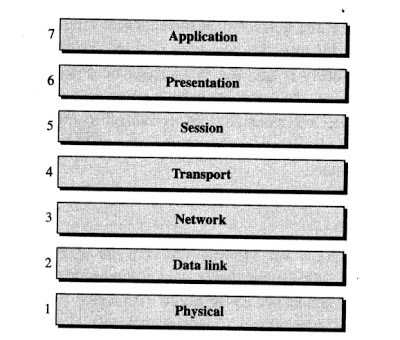
\includegraphics[scale=0.7]{osi_model.jpg}
\caption{Seven layers of the OSI network modell}
\label{addressing}
\end{figure}

\begin{etaremune}
\item Physical Layer

The physical layer defines the electrical and physical specifications of the data connection. It defines the relationship between a device and a physical transmission medium (e.g., a copper or fiber optical cable). 

\item Data Link Layer

The data link layer provides node-to-node data transfer - a reliable link between two directly connected nodes, by detecting and possibly correcting errors that may occur in the physical layer.

\item Network Layer

The network layer provides the functional and procedural means of transferring variable length data sequences (called datagrams) from one node to another connected to the same network. It translates logical network address into physical machine address. 

\item Transport Layer

The transport layer provides the functional and procedural means of transferring variable-length data sequences from a source to a destination host via one or more networks, while maintaining the quality of service functions.

\item Session Layer

The session layer controls the dialogues (connections) between computers. It establishes, manages and terminates the connections between the local and remote application. 

\item Presentation Layer

The presentation layer establishes context between application-layer entities. This layer provides independence from data representation (e.g., encryption) by translating between application and network formats.

\item Application Layer

The application layer is the OSI layer closest to the end user, which means both the OSI application layer and the user interact directly with the software application. This layer interacts with software applications that implement a communicating component.

\end{etaremune}

\section*{Explain encapsulation and de-capsulation in detail.}
In computer networking, encapsulation is a method of designing modular communication protocols in which logically separate functions in the network are abstracted from their underlying structures by inclusion or information hiding within higher level objects. 
1. Encapsulation (networking) - Wikipedia, the free encyclopedia
en.wikipedia.org\/wiki\/Encapsulation\_(networking)\cite[Encapsulation (networking)]{wikipedia}

\section*{Explain multiplexing and demultiplexing in detail.}
In telecommunications and computer networks, multiplexing (sometimes contracted to muxing) is a method by which multiple analog message signals or digital data streams are combined into one signal over a shared medium. The aim is to share an expensive resource. For example, in telecommunications, several telephone calls may be carried using one wire. The multiplexing divides the capacity of the low-level communication channel into several high-level logical channels, one for each message signal or data stream to be transferred. A reverse process, known as demultiplexing, can extract the original channels on the receiver side.


\section*{Explain addressing in the TCP/IP suite in detail.}

The TCP/IP protocol suited involves 4 different types of addressing:
\begin{enumerate}
\item Physical Address
\begin{itemize}
\item[-] Physical Address is the lowest level of addressing, also known as link address.
\item[-]  It is local to the network to which the device is connected and unique inside it.
\item[-] The physical address is usually included in the frame and is used at the data link layer.
\item[-] MAC is a type of physical address that is 6 byte (48 bit) in size and is imprinted on the Network Interface Card (NIC) of the device.
\item[-] The size of physical address may change depending on the type of network. Ex. An Ethernet network uses a 6 byte MAC address.
\end{itemize}

\item Logical Address
\begin{itemize}
\item[-] Logical Addresses are used for universal communication.
\item[-] Most of the times the data has to pass through different networks; since physical addresses are local to the network there is a possibility that they may be duplicated across multiples networks also the type of physical address being used may change with the type of network encountered. For ex: Ethernet to wireless to fiber optic. Hence physical addresses are inadequate for source to destination delivery of data in an internetwork environment.
\item[-]  Logical Address is also called as IP Address (Internet Protocol address).
\item[-] At the network layer, device i.e. computers and routers are identified universally by their IP Address.
\item[-] IP addresses are universally unique.
\item[-] Currently there are two versions of IP addresses being used, IPv4 - 32 bit address, and IPv6
\end{itemize}


\item Port Address
A logical address facilitates the transmission of data from source to destination device. But the source and the destination both may be having multiple processes communicating with each other.

\item Specific Address
\end{enumerate}

Each address is related to a specific layer in the TCP/IP network model architecture, as shown in Figure \ref{addressing}

\begin{figure}[!htp]
\centering
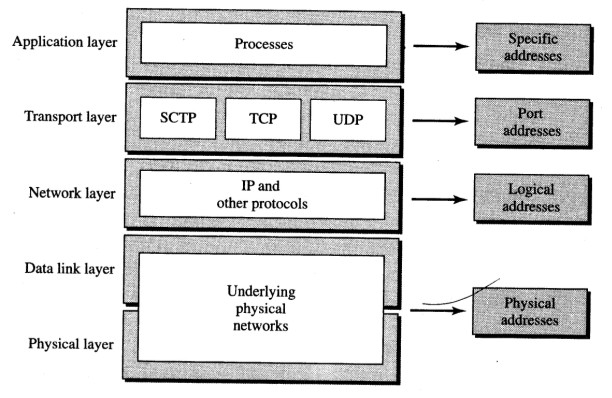
\includegraphics[scale=0.6]{NetworkModel3.jpg}
\caption{Addressing in TCP/IP model}
\label{addressing}
\end{figure}

\section*{Compare TCP/IP protocol suite with OSI model in detail.}

Following are some major differences between OSI Reference Model and TCP/IP Reference Model, with diagrammatic comparison shown in Figure \ref{tcpip_osi_comparison}.

\textbf{OSI(Open System Interconnection)}
\begin{itemize}
\item OSI provides layer functioning and also defines functions of all the layers
\item In OSI model the transport layer guarantees the delivery of packets
\item Follows horizontal approach
\item OSI model has a separate presentation layer
\item OSI is a general mode
\item Network layer of OSI model provide both connection oriented and connectionless service
\item OSI model has a problem of fitting the protocols in the model
\item Protocols are hidden in OSI model and are easily replaced as the technology changes
\item OSI model defines services, interfaces and protocols very clearly and makes clear distinction between them
\item It has 7 layers
\end{itemize}

\textbf{TCP/IP(Transmission Control Protocol / Internet Protocol)}

\begin{itemize}
\item TCP/IP model is more based on protocols and protocols are not flexible with other layers
\item In TCP/IP model the \\transport layer does not guarantees delivery of packets
\item Follows vertical approach.
\item TCP/IP does not have a separate presentation layer
\item TCP/IP model cannot be used in any other application
\item The Network layer in TCP/IP model provides connectionless service
\item TCP/IP model does not fit any protocol
\item In TCP/IP replacing protocol is not easy.
\item In TCP/IP it is not clearly separated its services, interfaces and protocols.
\item It has 4 layers
\end{itemize}

\begin{figure}[!htp]
\centering
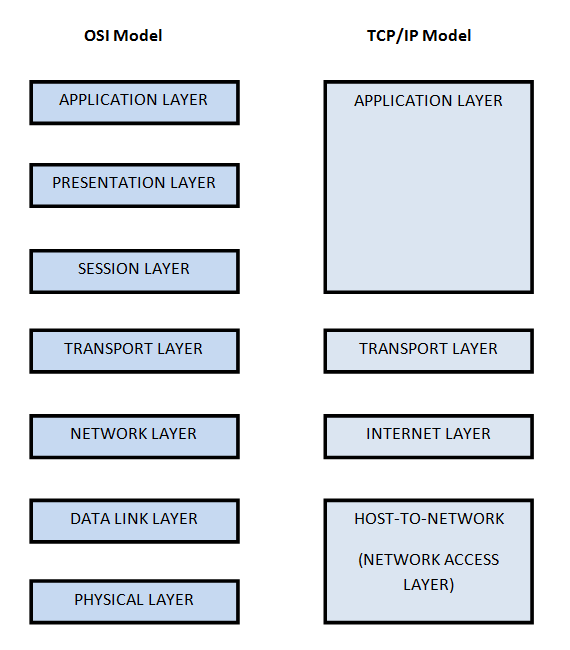
\includegraphics[scale=0.7]{tcpip_osi_comparison.png}
\caption{Diagrammatic Comparison between OSI Reference Model and TCP/IP Reference Model}
\label{tcpip_osi_comparison}
\end{figure}

\begin{thebibliography}{9}

\bibitem{lamport94}
 W. Stallings,
  \emph{Data and Computer Communications},
  Pearson Education,
  8th edition.

\bibitem{wikipedia}
  Wikipedia contributors,
  \emph{Wikipedia, The Free Encyclopedia}
  http://en.wikipedia.org/wiki/Encapsulation\_(networking)
  Accessed \today
  
\bibitem{google}
  Booksmart,
  \emph{Data Communication and Networking Standards}
  https://books.google.co.ke/books?id=G8ncBAAAQBAJ\&redir\_esc=y
  Accessed \today

\bibitem{wikipedia}
  Wikipedia contributors,
  \emph{Wikipedia, The Free Encyclopedia}
  http://en.wikipedia.org/wiki/OSI\_model
  Accessed \today

\bibitem{study_tonight}
  Study Tonight,
  \emph{Computer Networks}
  http://www.studytonight.com/computer-networks/comparison-osi-tcp-model
  Accessed \today  



\end{thebibliography}


\newpage
  \thispagestyle{empty}
  	\vspace*{\fill}
		\begin{center} 
		\textbf{THIS PAGE HAS BEEN INTENTIONALLY LEFT BLANK}
		\end{center}
	\vspace*{\fill}





 \end{document}


